\chapter{Results}

In this chapter we go through quantitative results on the datasets Buffy, 
Pascal and VideoPose (\secref{datasets}), analyzing behavior and design choices 
of our methods.  We also compare our models---CPS, ESM and LLPS---against 
competing models (\secref{competition}).  For much of the analysis we focus on 
upper and lower arms only---in particular, elbow and wrist localization 
accuracy.  The reasons for this are that (1) torso and head localization are 
near-perfect given a detected person \citep{deva2011}, (2) arms are the most 
interesting parts, involved in actions, hand-held objects and object-person 
interactions.


\section{Coarse-to-fine cascade evaluation}
 \begin{table}[tb]
\begin{center}
\begin{tabular}{|c|c|c|c|c|c|}
\hline
\multirow{3}{*}{cascade level}   & state        & \multicolumn{2}{|c|}{\# 
states in the}        &  \multirow{3}{*}{ } state space       & near-correct \\\cline{3-4}
 &       dimensions &original   & pruned        & reduction     &  lower arms  \\
 &       & space        & space & \%    & unpruned (PCP) \\

\hline
\hline
0        & 10x10x12      & 153600        & 1200 &        00.00 & 100  \\
\hline
1        & 10x10x24      & 72968 &      1140  &  52.50   & 76.6 \\
\hline
3        & 20x20x24      & 6704  & 642  &  95.64         & 72.3 \\
\hline
5        & 40x40x24      & 2682  & 671   & 98.25         & 70.5 \\
\hline 
7        & 80x80x24      & 492   & 492&          99.67   & 68.4 \\
\hline
\hline
detection pruning        & 80x80x24      & 492   & 492&          99.67   & 58.6 \\
%pruning         &       &       &&              &  \\
\hline
\end{tabular}


\caption[Coarse-to-fine cascade progression analysis.]{Coarse-to-fine cascade 
progression analysis. We show the progression of state spaces in the cascade, 
as well as reduction in the state space at each level (measuring efficiency), 
and in the last column, how many arm hypotheses remain closely matched, 
considering the closest match to groundtruth remaining from the unpruned 
hypotheses (measuring accuracy). }
\label{tab:c2f} 
\end{center}
\end{table}

In \tabref{c2f} we show the progress of our CPS model's coarse-to-fine cascade, 
in the Buffy dataset.
As explained in \secref{impl-details}, we start with a small state space and 
continue pruning and refining until we reach a somewhat fine $80 \times 80 
\times 24$ grid.  At the end of the cascade we are left with on average $492$ 
states for each part, $99.67\%$ fewer states than the complete $80 \times 80 
\times 24$. We see that after $1$ level the cascade, we have already pruned a 
large fraction of the state space away---roughly half.  This is intuitive 
because there are many easy decisions of states to reject based on even 
geometry alone, \eg the left elbow does not ever appear in the upper right 
corner of the person's bounding box.

As the cascade progresses, we do lose arm hypotheses close to the groundtruth 
arms---last column of \tabref{c2f}.  However, the percent of hypotheses close 
to groundtruth after the cascade process is still higher than any current 
system's accuracy on lower arms (see \tabref{res-table}).  Thus this number 
($68.4 \%$) is an upper bound on how well we could do with our small, pruned 
set of states.

To verify that our pruning is better than heuristic pruning, we compare to 
heuristic pruning in \tabref{c2f}, last row.  The heuristic here is to sample 
states proportional to their unary potential scores (\ie, HoG limb detectors), 
with non-max suppression.  At the same number of states sampled as we our left 
with via our cascade, the heuristic pruning misses $10\%$ more lower arm 
hypotheses.

Finally, it could be that case that the benefits of our rich features in the 
last stage make discrepencies in accuracy of pruning strategies neglible.  In 
other words, even the pruning heuristic retains $58.6\%$ of lower arms in its 
hypothesis set, and it is possible that it could perform equally well at 
final-level prediction when using the same features as CPS.  We see in 
\figref{cascade-vs-pruning} that this is not this is not the case.  CPS 
performs $5-10\%$ better than simple detector pruning coupled with the rich 
features we use in CPS.  This makes a strong case that the CPS state filtering 
strategy is important.

\begin{figure}[tb]
\begin{center}
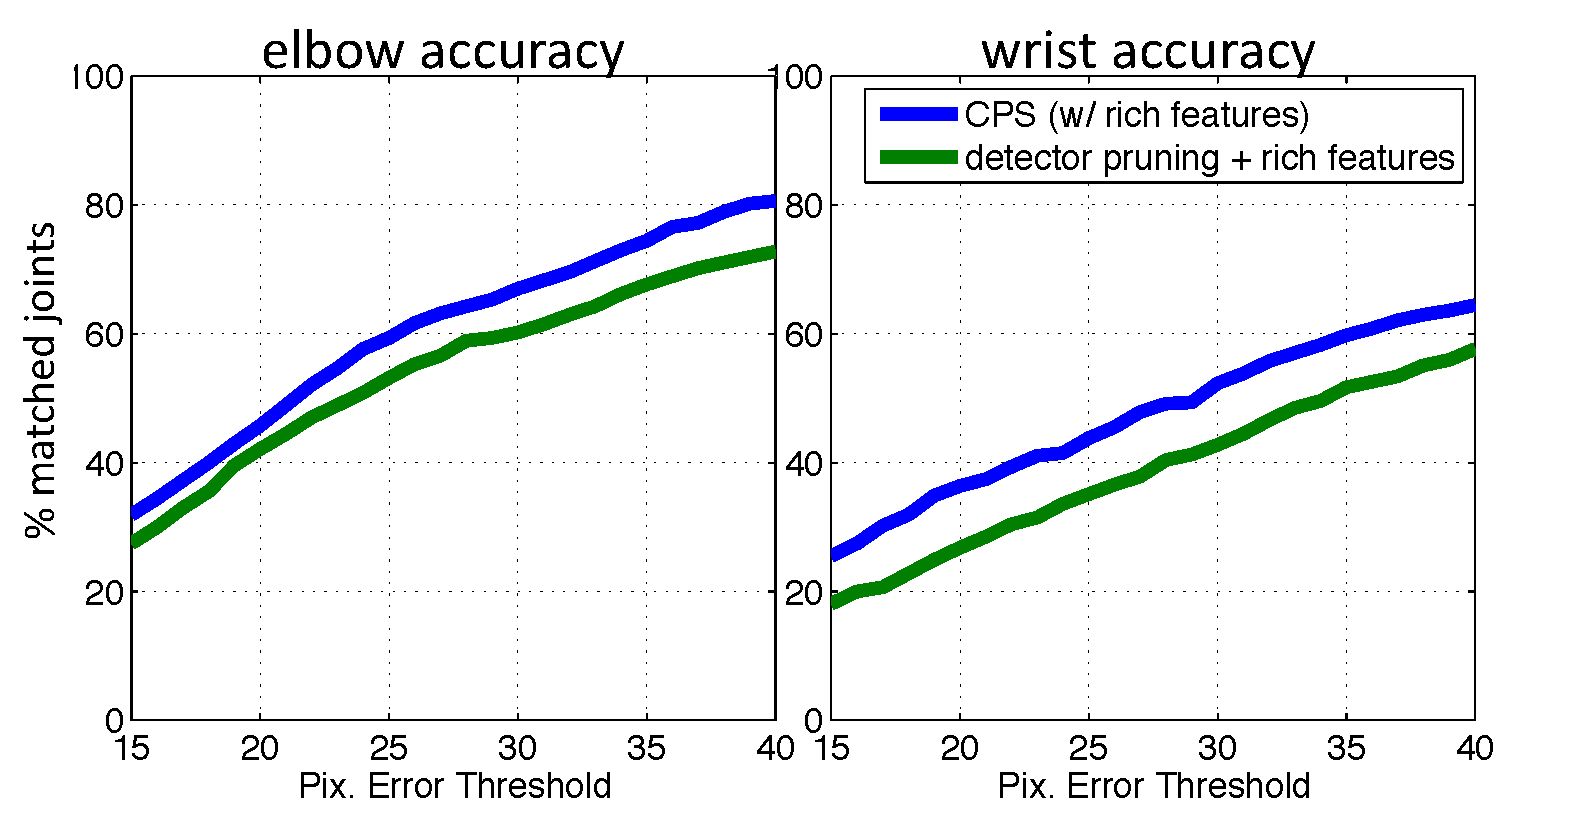
\includegraphics[width=0.99\textwidth]{figs/cascade-vs-pruning.pdf}
\caption[Cascade versus heuristic pruning.]{Cascade versus heuristic pruning.  
Here we see that our cascade progression, coupled with a rich set of features 
does better than heuristic pruning with the same rich features used afterwards.  
This indicates that not only do the rich features matter, but also the quality 
of the states retained from CPS.}
\label{fig:cascade-vs-pruning}
\end{center}
\end{figure}


\section{Feature analysis}
\begin{figure}[tb]
\begin{center}
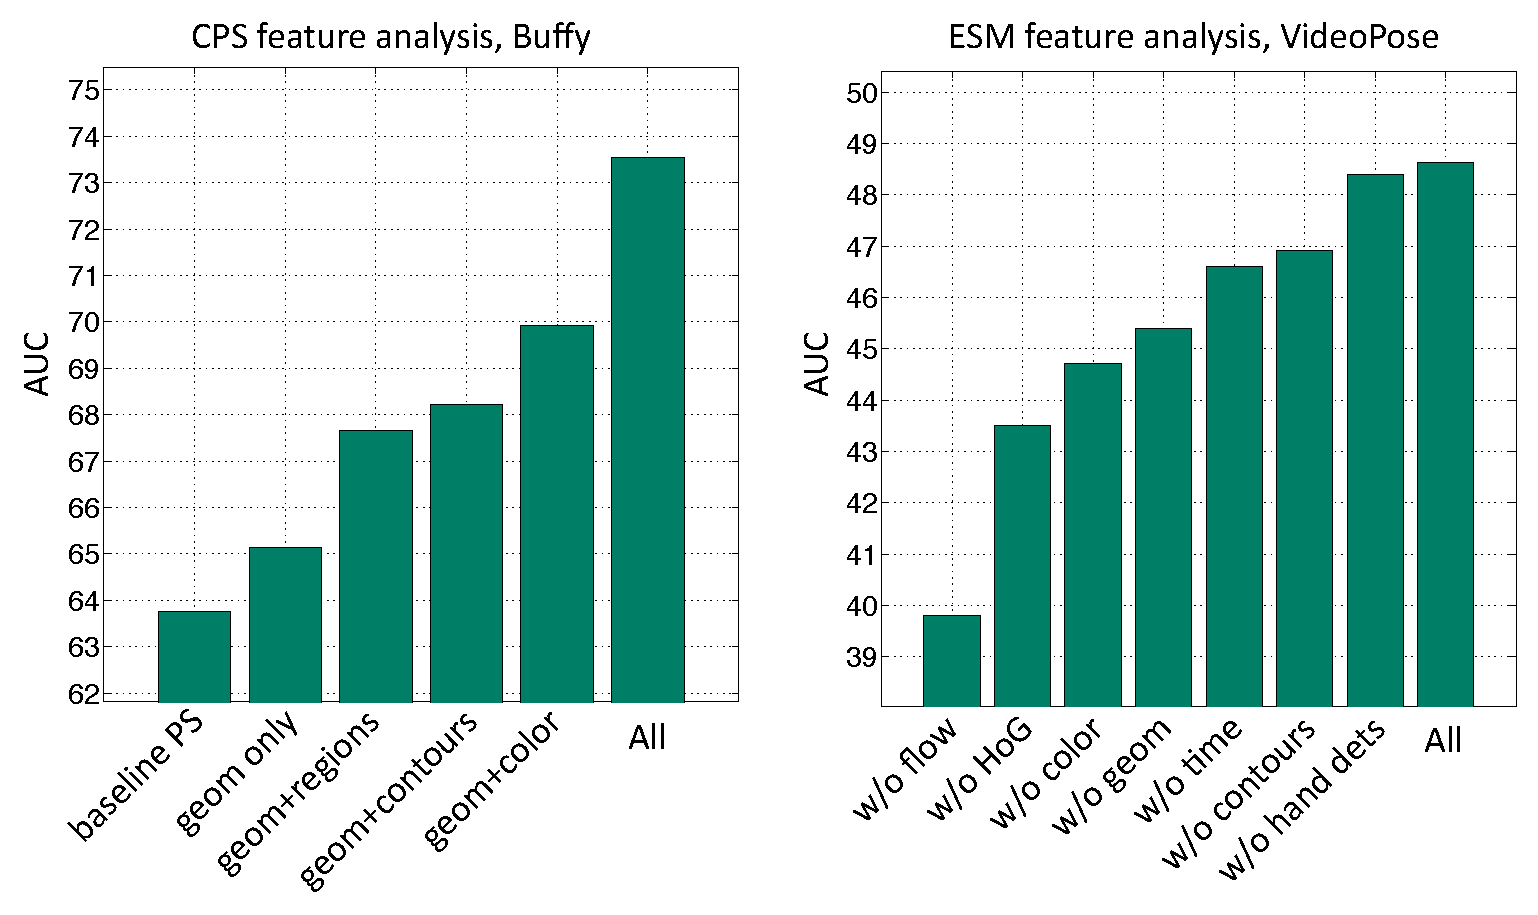
\includegraphics[width=0.99\textwidth]{figs/ablative-bars}
\caption[Feature analysis.]{Feature analysis.  On the left, we observe how 
adding features contributes to final system performance of CPS on Buffy, 
measuring the Area Under the Curve of pixel error distance.  On the right, we 
observe how removing single feature modalities from our Ensemble of Stretchable 
Models affects performance.}
\label{fig:ablative}
\end{center}
\end{figure}

One of the main contributions of this thesis was technical innovations that 
allow us to include ``everything and the kitchen sink'' (in the house of vision 
features).  At this point we wish to verify that the work done implementing, 
computing and learning parameters for features makes a difference in 
performance.  This is actually quite difficult to do in general, because it is 
computationally infeasible to explore the combinatorially many possibilities of 
feature sets, whose interactions between modalities are significant.  We 
analyze the importance of of features by grouping them by modality, and adding 
or removing them from our full systems in turn, measuring the change in 
performance.

In \figref{ablative} we do a feature analysis for CPS (left) and ESM (right), 
grouping features by coarse modalities.  The first important thing to note is 
that, by and large, the rich features we include over standard edge template 
and geometry information help.  For CPS, we see that including rich features of 
simple geometry alone helps performance, in particular pairwise cues such as 
color and contours that we intractable to compute without a cascade approach.  
An interesting except is the region based features working in isolation 
actually {\em hurt} performance slightly on the test set.  However, all 
features together do significantly better than any one feature modality on top 
of the standard geometric information.

On the right side of \figref{ablative}, we do an ablative analysis of our ESM 
model.  Interestingly, the hand detector features slightly hurt system 
performance on the test set, contrary to training and validation procedures.  
The most important individual feature modality was optical flow, which gives us 
a fairly good estimate of foreground/background separation in many video 
frames.  Importantly, many of these feature modalities are not used in pose 
estimation models because they require joint interactions which lead to loopy, 
cyclic models.


\section{System results}\label{sec:system-results}
In this section we analayze end-to-end system results, using the publicly 
available code for our systems and competitors, for reproducibility's sake.
\begin{table}[tb]
\begin{center}
\begin{tabular}{| c | c | c | c | c |c | c | c |}
\hline
---&\multicolumn{2}{c|}{MoviePose} & \multicolumn{2}{c|}{Buffy v2.1} & \multicolumn{2}{c|}{Pascal Stickmen} & all \\ 
\hline
method & uarms & larms & uarms & larms & uarms & larms & mean \\ 
\hline 
\cite{andriluka09} & --- & --- & 79.3 & 41.2 & --- & --- & 60.3\\ 
\cite{eichner-tr} & 90.40 &52.85 & 92.77	& 53.40	& 67.92	& 30.56	& 57.19 \\
\cite{deva2011} &  94.05 &	67.08 &	92.77 & 65.53 & 65.83 & 37.92 & 70.53 \\
CPS & 93.95 &	52.12 &	95.11 &	67.02 &	86.39 &	59.17 &	75.62 \\
LPPS & 95.57 & 71.85 & 88.94 & 70.64 & 68.61 & 44.58 & 73.37 \\
\hline 
mean pose & 78.25	& 33.22	& 93.19	& 43.83	& 72.92	& 34.03	& 59.24 \\
mean cluster prediction & 95.13	& 63.73	& 96.81	& 70.85	& 85.83	& 53.75	& 77.68 \\
\hline 
\end{tabular}


%----- old table --------------%

\out{
\begin{tabular}{| c | c | c |c | c | c |}
\hline
PCP & \multicolumn{2}{c|}{Buffy v2.1} & \multicolumn{2}{c|}{Pascal Stickmen} & \\ 
\hline
method & upper arms & lower arms & upper arms & lower arms & mean \\ 
\hline 
\cite{andriluka09} & 79.3 & 41.2 & --- & --- & 60.3\\ 
\cite{eichner09} & 82.8 & 59.8 & 73.8 & 41.5 & 64.5\\ 
\cite{deva2011} & 96.6 & 70.9 & 84.2 & 45.8 & 74.4 \\
CPS & 95.3 & 63.0 & 81.5 & 53.9 & 73.4\\ 
LPPS & 90.0 & 62.6 & 83.9 & 47.1 & 70.9\\ 
\hline 
\end{tabular}
}

\caption[PCP evaluation.]{PCP Evaluation of single frame pose estimation. PCP 
is a fairly loose measure of accuracy and only reveals one precision operating 
point.  We include the measure for historical reasons; for a more detailed 
picture see \figref{results-buffy-pascal}.}
\label{tab:res-table} 
\end{center}
\end{table}


\subsection{Single frame pose estimation}
\begin{figure}[tb]
\begin{center}
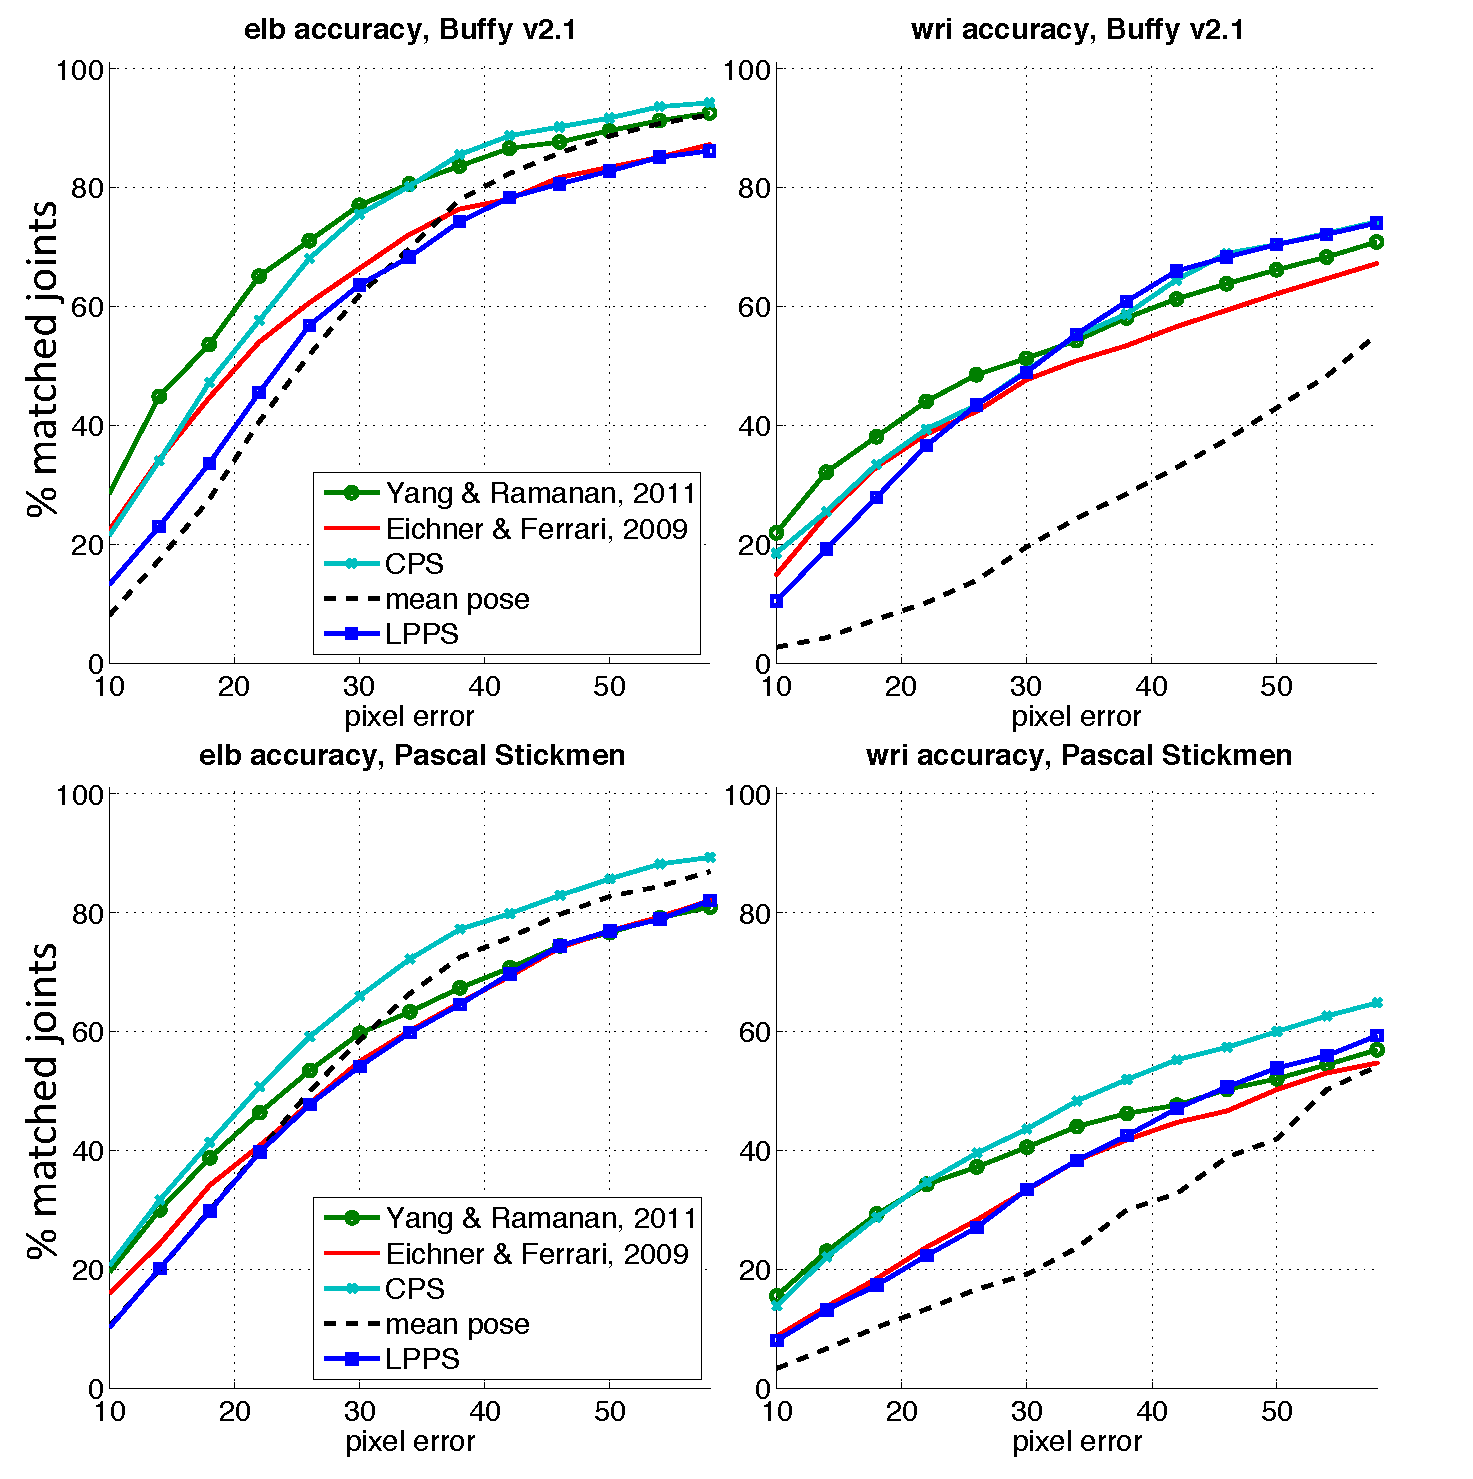
\includegraphics[width=1.00\textwidth]{figs/results-buffy-pascal.pdf}
\caption[Single frame pose estimation results.]{Single frame pose estimation 
results.  Shown are our single frame models CPS and LPPS against 
state-of-the-art competitor models (\secref{competition})}.
\label{fig:results-buffy-pascal}
\end{center}
\end{figure}
The performance of all single-frame models are shown on the Buffy and Pascal 
datasets in \figref{results-buffy-pascal}.  We see that in general, CPS and 
\citet{deva2011} outperform the rest, with CPS performing strictly better on 
Pascal.  LPPS and \citet{eichner09} are also comparable, trading off better 
performance in different regimes of precision.   However, absolute performance 
localization accuracy is only one way to measure the quality of a model---see 
\secref{discussion} for more discussion.

Surprisingly, the ``mean pose'' baseline outperforms some models elbow 
localization accuracy in some regimes, in particular on the Pascal dataset.  
This is an indication of either the difficulty or boringness (lack of pose 
variation) in these datasets, or a combination of both.  In fact, the 
scatterplots in \figref{dataset-scatterplots} do show that most elbows are very 
tightly grouped in these single frame datasets. 

We also report PCP scores in~\tabref{res-table}.  Comparing the induced ranking 
of methods by \tabref{res-table} and \figref{results-buffy-pascal}, we see that 
PCP does not give a complete story of performance.

\subsection{Video pose estimation}
\begin{figure}[tb]
\begin{center}
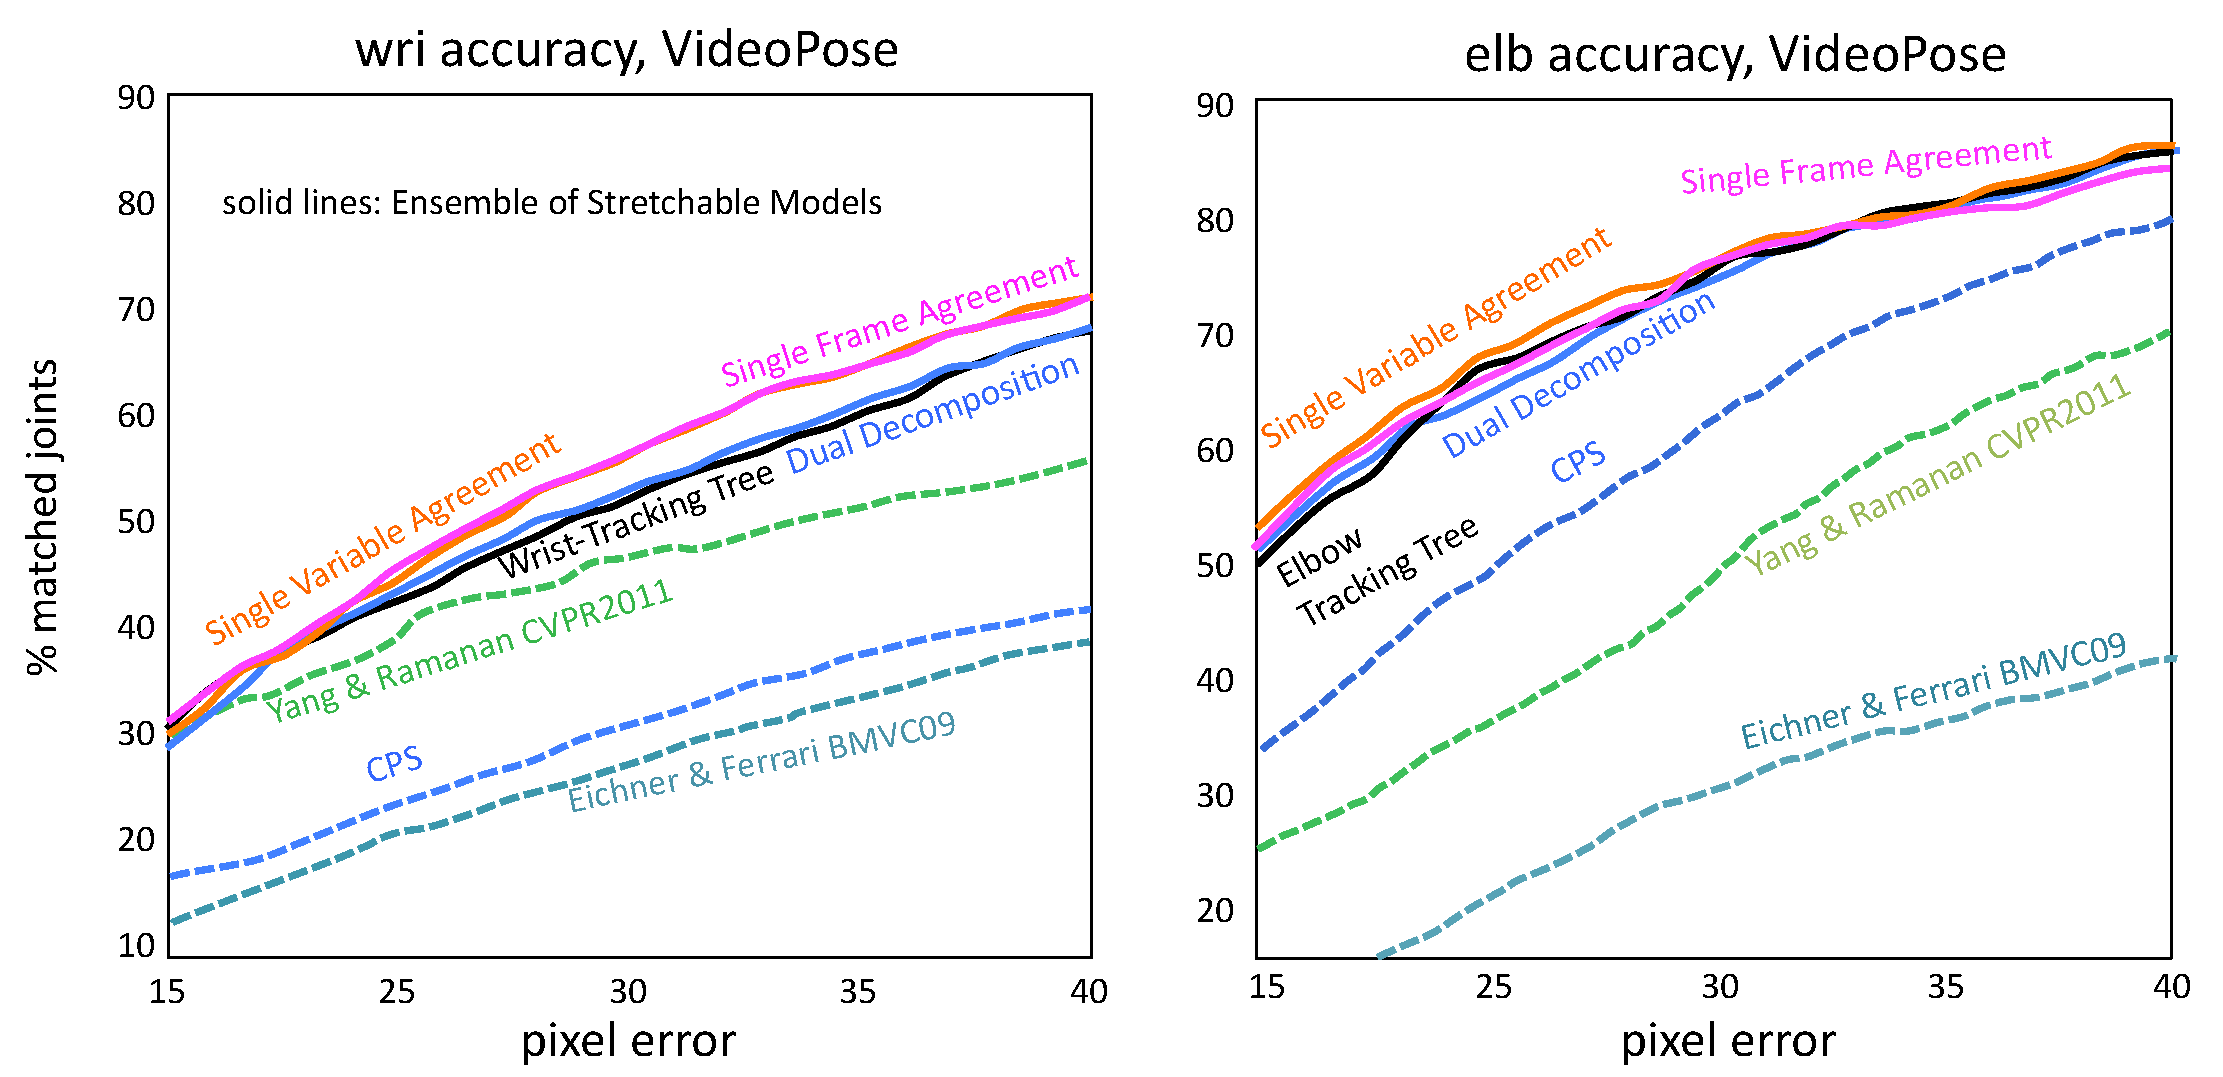
\includegraphics[width=1.00\textwidth]{figs/results-vpose.pdf}
\caption[Video pose estimation results.]{Video pose estimation results.  Shown 
are our single frame model CPS, various forms of agreement for Ensembles of 
Stretchable Models, and other single frame competitors.}
\label{fig:results-vpose}
\end{center}
\end{figure}

Quantitative results for pose estimation in video are shown 
in~\figref{results-vpose}.  All three methods we explore for inference in our 
pose estimation video model (Ensemble of Stretchable Models) outperform the 
state-of-the-art single-frame methods by a significant margin.  Using just a 
single one of our Stretchable Model trees already does significantly better 
than single frame models.  This shows the usefulness of our stretchable model 
(joint-centric) representation of pose, as well as some of the rich pairwise 
interactions we use that other models do not.  It is important to note that 
previous work has found the incorporating time persistence into models actually 
{\em hurt } performance~\citep{posesearch,weisssapp10}---hence single frame 
models are the most competitive models for which to compare.

Furthermore, we explore the different agreement methods discussed 
in~\secref{stretchable-inference}.  From \figref{results-vpose}, we see that 
the very fast, approximate decoding schemes (A single tree and $SV$ require 
only a single inference pass) were comparably accurate to more expensive 
methods ($SF$ takes about $2\times$ as long while we ran $DD$ for $500\times$ 
iterations, each requiring inference in each submodel)\footnote{Specifically, 
running inference in all 6 models sequentially takes about 16 seconds per 30 
frame clip (trivial to parallelize) on a Intel Xeon CPU, E5450 @ 3.00GHz.  $SF$ 
inference takes an additional 19 seconds.}. We found two important trends: (1) 
On average, completely decoupled inference ($Independent$) was consistently 
about 0.75-1.5\% worse than the inference methods that aggregated information 
across models, and (2) solving {\em partial} agreement problems {\em exactly} 
($SV, SF$) performed better than solving {\em complete} agreement {\em 
approximately} with Dual Decomposition. 

The absolute accuracy values are also a testament to the difficulty of the 
dataset: At the tightest matching criterion, we only correctly localize half 
the elbows.  This suggests that there is plenty of future progress to be made 
on this dataset, and in this domain in general.


